\section{Methoden und Durchführung}
Zuerst soll die Kennlinie der Diode bestimmt werden. Dazu wird diese nach \cref{Aufbau} gemessen. Dabei wird die die Leistung der Mikrowellenstrahlung in Spannung umgewandelt. Dies wird auch in allen weiteren Messungen verwendet, da sich die Spannung einfacher direkt messen lässt.

\begin{figure}[h]
	\centering
	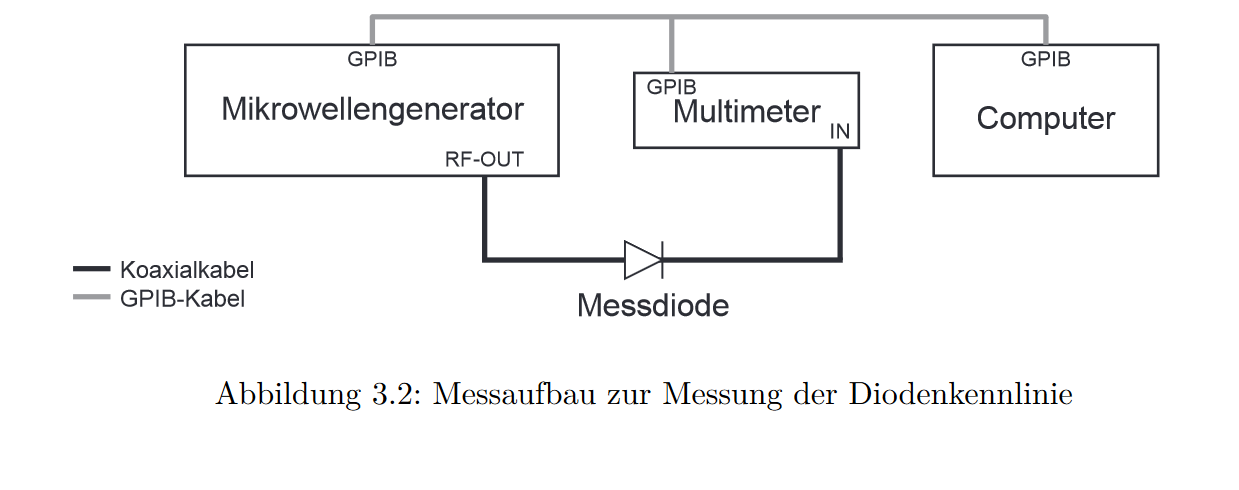
\includegraphics[scale=0.4]{../Diode_Aufbau.PNG}
	\caption{Skizze des Versuchaufbaus}
	\label{Aufbau}
\end{figure}

Zuletzt sollen in zwei verschiedenen Koaxialkabeln stehende Wellen erzeugt und die Resonanzfrequenzen, bei denen die stehenden Wellen beobachtet werden, gemessen werden. Aus den Abständen zwischen den Resonanzen soll anschließend mit \cref{eq:c} die Ausbreitungsgeschwindigkeit der Welle im Kabel berechnet werden.
\begin{equation}
c = 2l(f_{n+1} - f_n)
\label{eq:c}
\end{equation}
Zuletzt soll dann mit \cref{eq:er} die relative Permittivität bestimmt werden.
\begin{equation}
\epsilon_r = \left( \frac{c_0}{c}\right) ^2
\label{eq:er}
\end{equation}

\section{Ergebnis}
\subsection{Kennlinie}
Zuerst wird die Kennlinie der Diode bestimmt. Diese wird in \cref{fuck_scidavis} dargestellt. Dabei wird mit einer e-Funktion gefittet, durch die beschrieben wird, welche Leistung in wie viel Spannung umgewandelt wird. 

\begin{figure}[h]
	\centering
	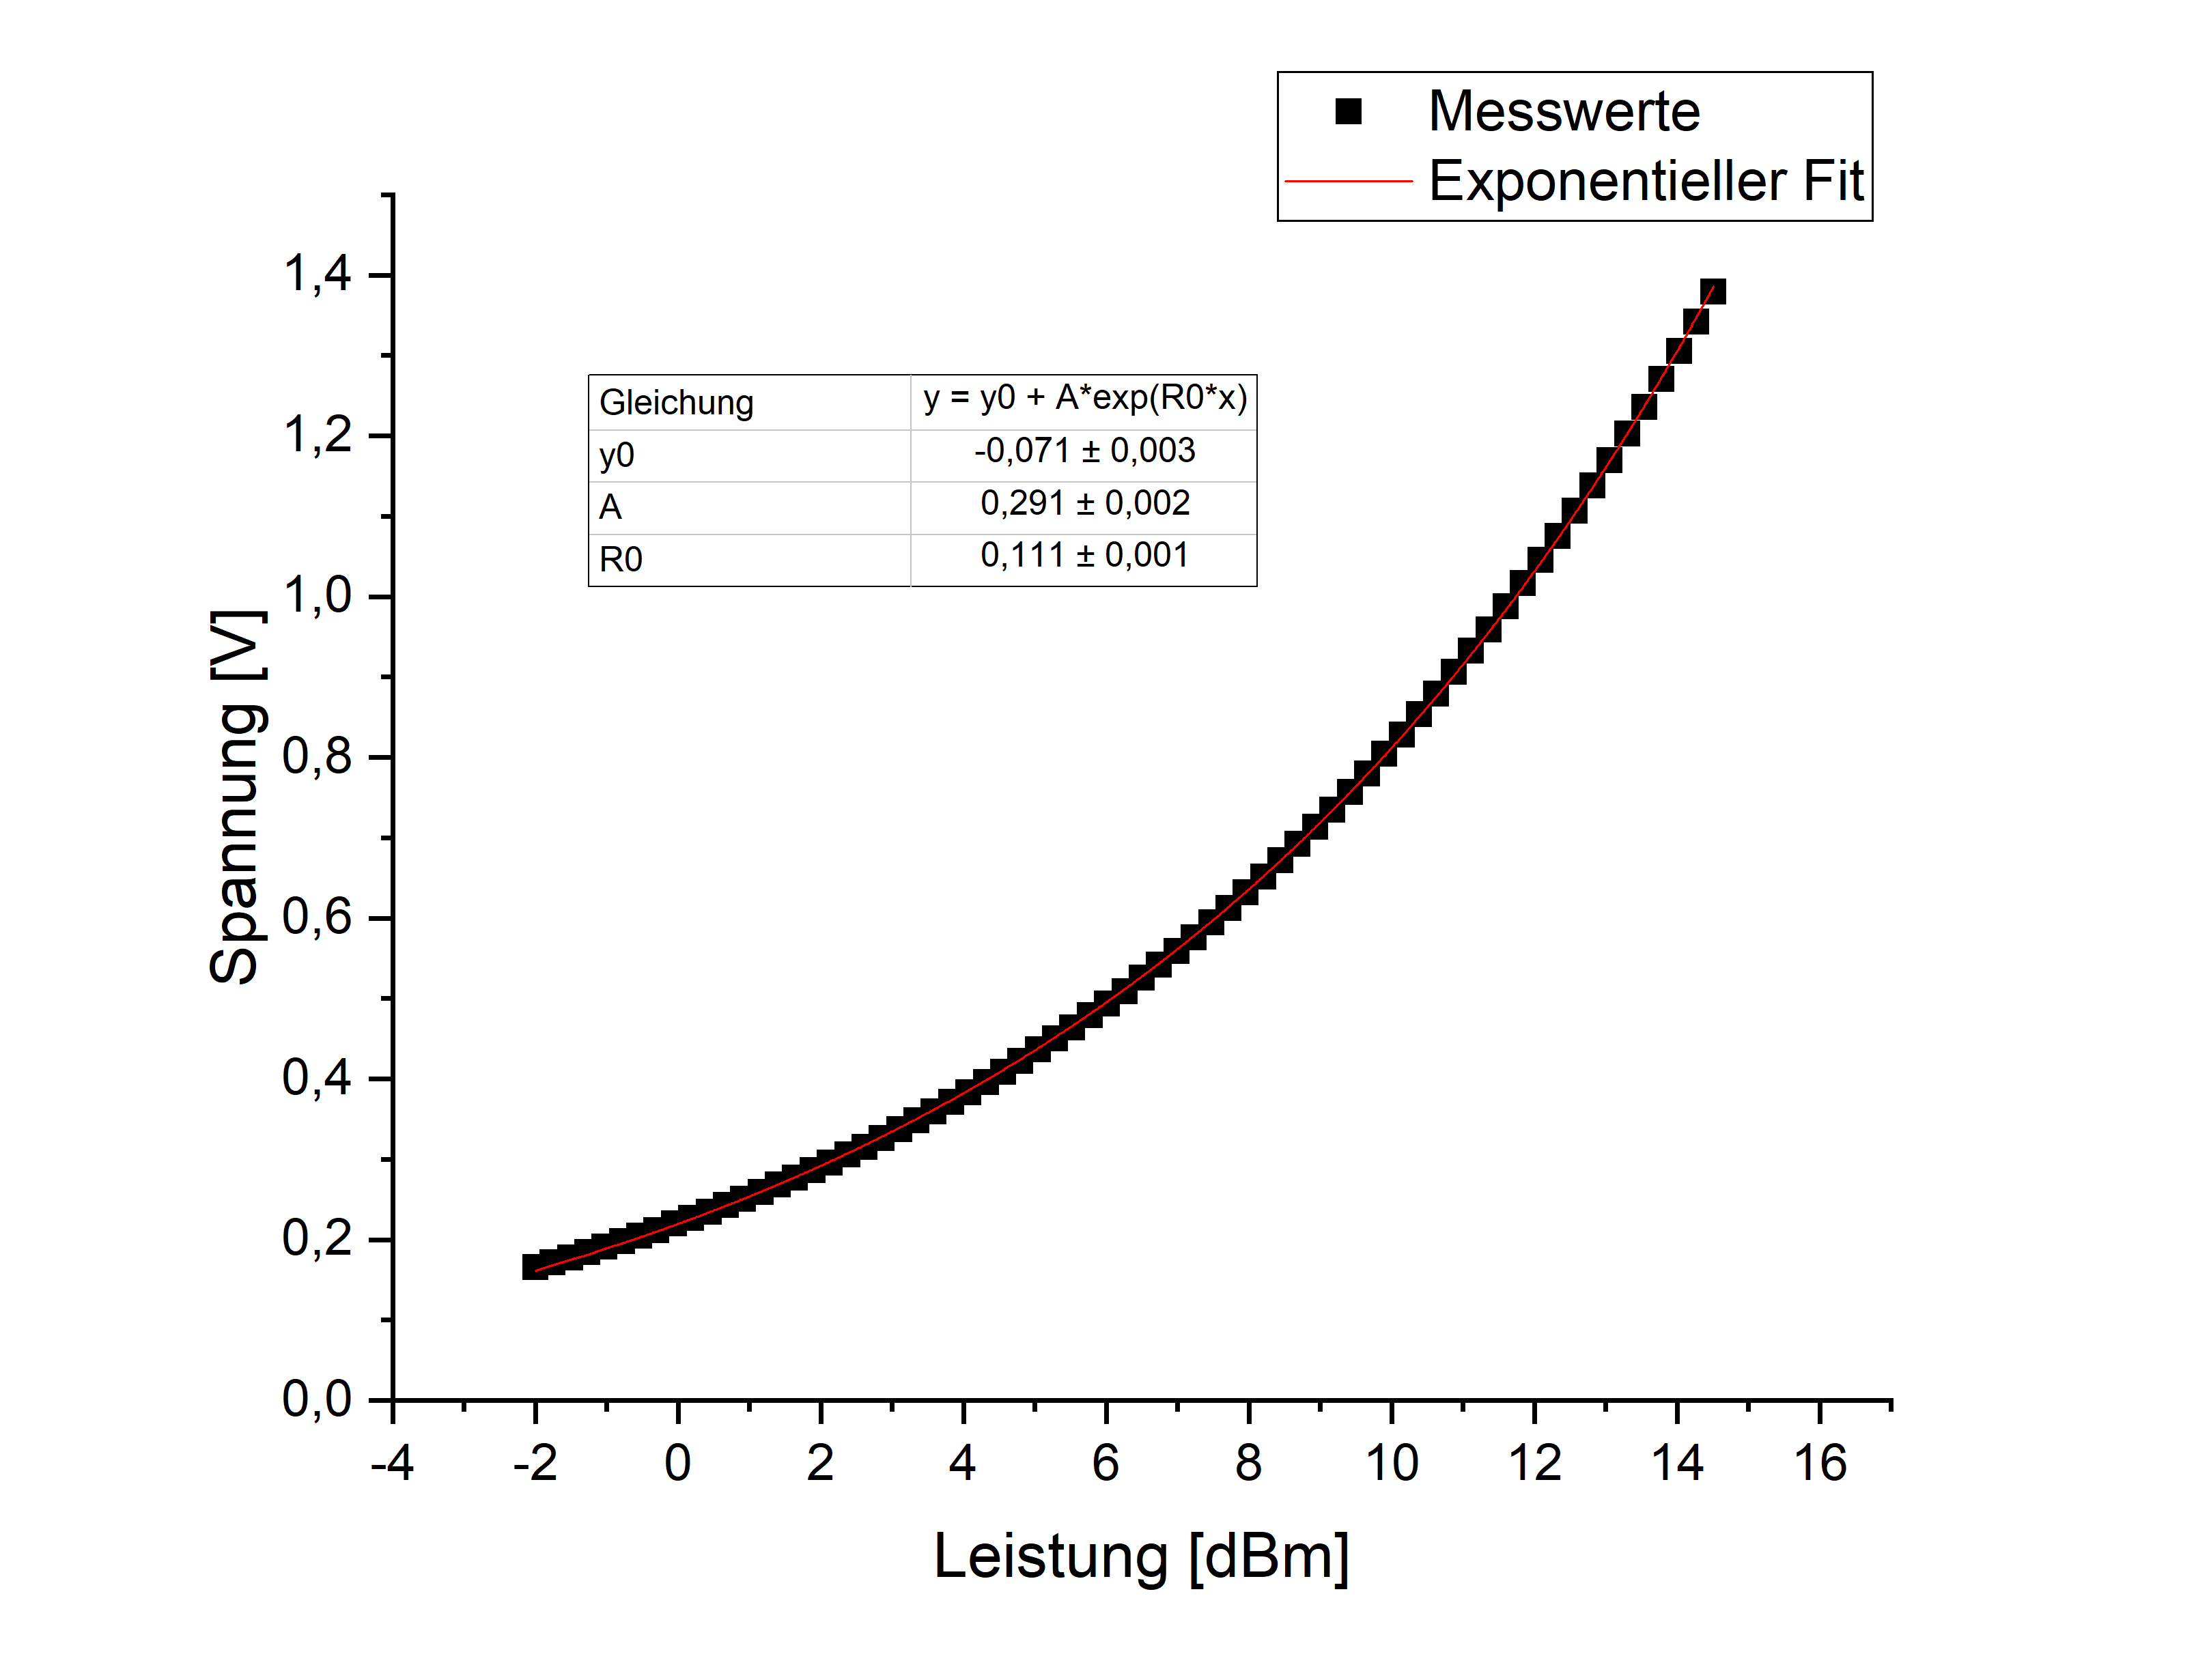
\includegraphics[scale=0.4]{../fuck_scidavis.png}
	\caption{Kennlinie der Diode}
	\label{fuck_scidavis}
\end{figure}

\subsection{Ausbreitungsgeschwindigkeit und relative Permittivität}
Im letzten Abschnitt werden Lichtgeschwindigkeit und Permittivität zwei verschiedener Koaxialkabel bestimmt. In \cref{gleich} sind die Messergebnisse für die Messung mit Kabel 1 sowohl für offenes Kabelende als auch für kurzgeschlossenes Kabelende dargestellt. Dabei ist die Leistung in dBm gegen die Frequenz in GHz aufgetragen.